%----------------------------------------------------------------------
\documentclass[xcolor=svgnames]{beamer} %, handout
\usetheme{lined}
\usepackage{array}
\usepackage{amsmath}
\usepackage{amssymb}
\usepackage{amsthm}
\usepackage{bbm}
\usepackage[utf8]{inputenc}
\usepackage[T1]{fontenc}
\usepackage{cmbright}   
\usepackage{times}
\usepackage{geometry}
\usepackage[spanish]{babel}
\usepackage{multicol}
\usepackage{tcolorbox}

\usepackage{algorithm2e}

%\usepackage{psfrag}
\usepackage{graphicx}
\usepackage{color}
\usepackage{floatflt}
\usepackage{fancybox}
\usepackage{tabularx}
%\usepackage[all]{xy}
\usepackage{color}
\usepackage{siunitx} % para \degree



\usepackage{tikz}
\usetikzlibrary{positioning}




%\usepackage[most]{tcolorbox}


\theoremstyle{plain}
\newtheorem{definicion}{Definición}



\definecolor{redUnq}{rgb}{.7,.1,.1}
\definecolor{redUnq2}{rgb}{.5,.1,.3}

\mode<presentation>{
	%\usetheme{Boxes}
	%\usecolortheme[RGB={237,132,8}]{structure}
	%\usecolortheme[RGB={205,173,0}]{structure}
	\usecolortheme[RGB={100,10,10}]{structure}

	%\beamertemplateshadingbackground{SteelBlue!70}{Honeydew!10}
	%\usetheme{Warsaw}
	%\usecolortheme{default}
	\usetheme{Singapore}
	%\usetheme{Lined}
	%\usetheme[height=7mm]{Rochester} 
	\setbeamerfont{title}{shape=\bfseries,family=\rmfamily}
	%\usefonttheme[onlylarge]{structuresmallcapsserif}
	%\usefonttheme[onlysmall]{structurebold}
	\setbeamercolor{title}{fg=redUnq,bg=gray!40}
	\usefonttheme{professionalfonts}
	\setbeamercovered{highly dynamic}
	\setbeamercovered{transparent=10}
	\setbeamertemplate{navigation symbols}{}
	\colorlet{structure}{redUnq}

	\setbeamertemplate{frametitle}[default][left]
}

\definecolor{verzul}{rgb}{0, 0.5,0.5}

\renewcommand{\textbf}[1]{{\bfseries\textcolor{redUnq2}{#1}}}
\renewcommand{\emph}[1]{{\em\textcolor{redUnq2}{#1}}}

\setlength{\parindent}{0pt}
\theoremstyle{definition}
\newtheorem{ejem}{Ejemplo}
\newtheorem{defi}{Definición}
\newtheorem{ejer}{Ejercicio}
\newtheorem{prop}{Propiedad}
\newtheorem{lema}{Lema}
\newtheorem{teor}{Teorema}
\newtheorem{coro}{Corolario}

 

\newcommand{\Rset}{\mathbbmss{R}}
\newcommand{\Cset}{\mathbbmss{C}}
\newcommand{\PD}[2]{\frac{\partial #1}{\partial #2}}
\DeclareMathOperator{\tr}{tr}
\DeclareMathOperator{\adj}{adj}
\DeclareMathOperator{\rango}{rango}

\newenvironment{Boxedminipage}%
{\begin{Sbox}\begin{minipage}}%
{\end{minipage}\end{Sbox}\fbox{\TheSbox}}



\title{Métodos Numéricos - Clase 3}
  \logo{
\includegraphics[scale=0.25]{logoUnq} }
\author{Ulises Bussi- Javier Portillo}
%\institute{\scalebox{2}{\includegraphics[scale=0.1]{mdp02.jpg}}} %{Departamento de Ciencia y Tecnología\\ Universidad Nacional de Quilmes\\ }
\date{ $1^\circ$ cuatrimestre 2020} 


%%%%%%%%% Para que al comenzar una section aparezca el Contenido
%\AtBeginSection[]
%{
%  \begin{frame}
%    \frametitle{Contenidos de la Presentación}
%    \tableofcontents[currentsection]
%  \end{frame}
%}




\begin{document} 


\begin{frame} %\thispagestyle{empty}
	\titlepage
\end{frame}


\section{Introducción}
\begin{frame}
\frametitle{Métodos Abiertos.}

Métodos para encontrar raices de funciones de forma numérica (sí, también).\vspace{10pt}


\begin{tcolorbox}
  \begin{center}
 	Más efectivos computacionalmente.
  \end{center}
\end{tcolorbox} \vspace{20pt}
\pause


$"$Encuentra$"$ raices sin necesidad de un intervalo cerrado.



\end{frame}




\begin{frame}
\frametitle{Métodos Abiertos.}
\textbf{Consideraciones:}
\begin{itemize}
\item Encuentran aproximadamente el valor de la raiz.
\item Requieren una condición inicial.
\item Pueden tener problemas de convergencia.

\end{itemize}
\pause

\textbf{Metodos:}
\begin{itemize}
\item Punto fijo.
\item Newton-Raphson.
\item Método de la Secante.

\end{itemize}

\end{frame}






\section{Iteración de Punto Fijo}

\begin{frame}
\frametitle{Iteración de Punto Fijo}

\begin{tcolorbox}
\textbf{Idea}
	Dada $f(x)=0$ convertirlo a la forma $g(x) = x$ y dado un $x_0$
	calcular $x_1 = g(x_0)$

\end{tcolorbox}
\begin{minipage}{.45\linewidth}
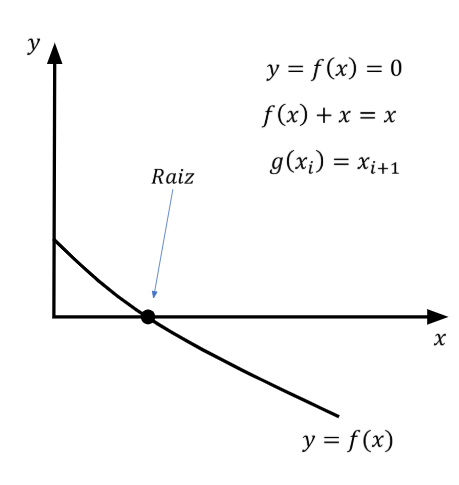
\includegraphics[width=\linewidth]{FixedPoint/fixed1.PNG} 

\end{minipage}  \begin{minipage}{.45\linewidth}
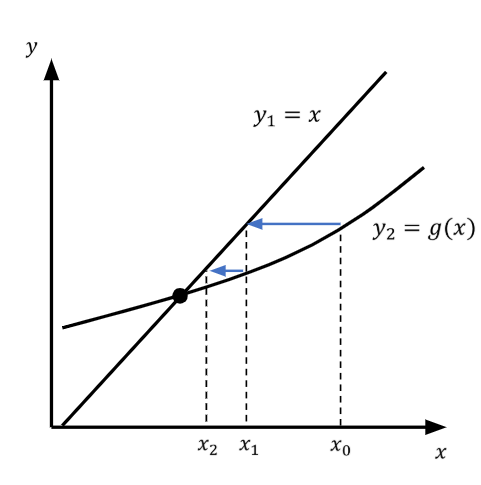
\includegraphics[width=\linewidth]{FixedPoint/fixed2.PNG} 

\end{minipage}



\end{frame}

\subsection{Ejemplo Punto Fijo}


\begin{frame}
\frametitle{Ejemplo: Punto Fijo}

Supongamos que queremos hallar la raiz de $f(x) = e^{-x} -x$



\begin{minipage}{.45\linewidth}
\includegraphics[width=\linewidth]{fp_example/f.png} 

\end{minipage} $\rightarrow$  \begin{minipage}{.45\linewidth}
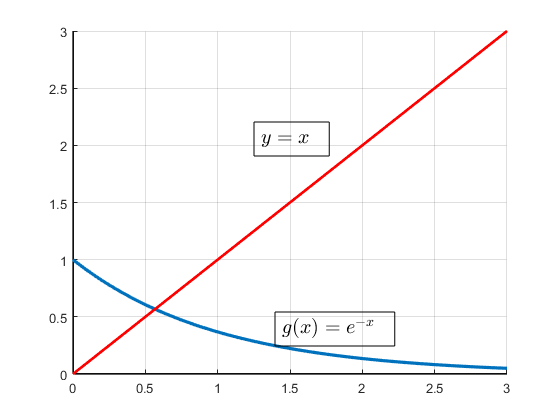
\includegraphics[width=\linewidth]{fp_example/g.png} 
\end{minipage}

$$g(x) = e^{-x}$$
\end{frame}



%iter 1
\begin{frame}
\frametitle{Ejemplo: Punto Fijo}

Supongamos que queremos hallar la raiz de $f(x) = e^{-x} -x$,
damos una condición inicial $x_0=2$


\begin{minipage}{.45\linewidth}
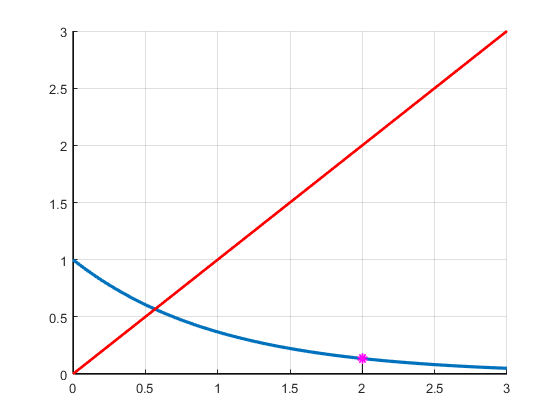
\includegraphics[width=\linewidth]{fp_example/iter1.png} 

\end{minipage} \begin{minipage}{.45\linewidth}
$$ x_1 = g(2) = e^{-2} = 0.1353$$

$$e_r = \frac{|0.1353-2|}{|0.1353|} = 13.78$$
\end{minipage}
\end{frame}

%iter 2
\begin{frame}
\frametitle{Ejemplo: Punto Fijo}

Supongamos que queremos hallar la raiz de $f(x) = e^{-x} -x$,
damos una condición inicial $x_0=2$


\begin{minipage}{.45\linewidth}
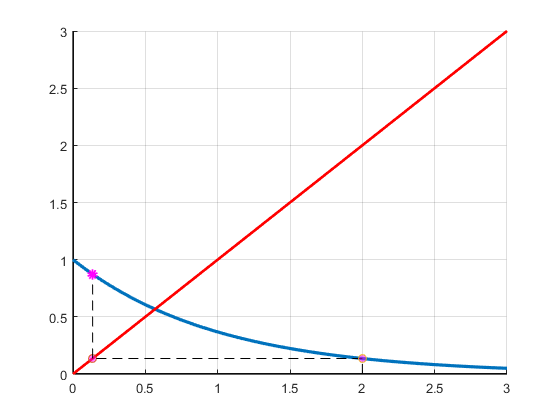
\includegraphics[width=\linewidth]{fp_example/iter2.png} 

\end{minipage}  \begin{minipage}{.45\linewidth}
$$ x_2 = g(0.1353) = 0.8734$$

$$e_r = \frac{|0.8734-0.1353|}{|0.8734|} = 0.8451$$
\end{minipage}
\end{frame}


%iter 3
\begin{frame}
\frametitle{Ejemplo: Punto Fijo}

Supongamos que queremos hallar la raiz de $f(x) = e^{-x} -x$,
damos una condición inicial $x_0=2$


\begin{minipage}{.45\linewidth}
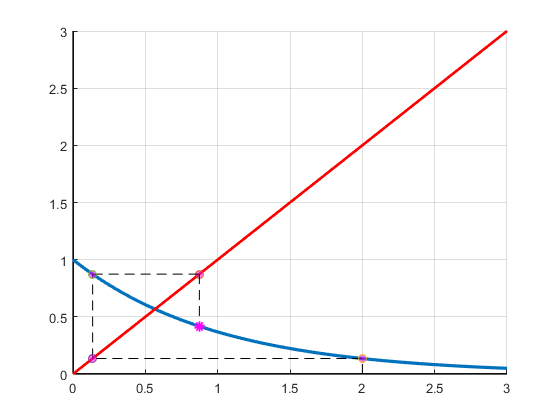
\includegraphics[width=\linewidth]{fp_example/iter3.png} 

\end{minipage}  \begin{minipage}{.45\linewidth}
$$ x_3 = g(0.8734) = 0.4175$$

$$e_r = \frac{|0.4175-0.8734|}{|0.4175|} = 1.0919$$
\end{minipage}
\end{frame}

%iter 4
\begin{frame}
\frametitle{Ejemplo: Punto Fijo}

Supongamos que queremos hallar la raiz de $f(x) = e^{-x} -x$,
damos una condición inicial $x_0=2$


\begin{minipage}{.45\linewidth}
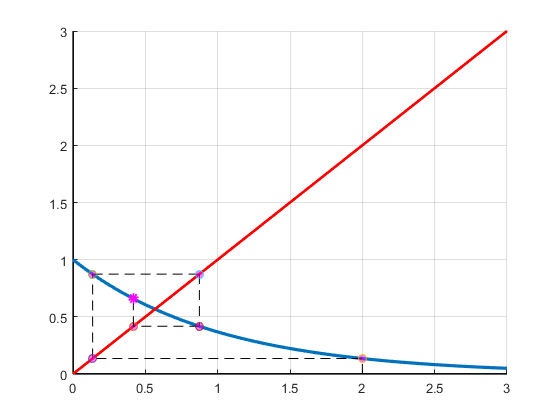
\includegraphics[width=\linewidth]{fp_example/iter4.png} 

\end{minipage}  \begin{minipage}{.45\linewidth}
$$ x_4 = g(0.4175) = 0.6587$$

$$e_r = \frac{|0.4175 - 0.6587|}{|0.6587|} = 0.3661$$
\end{minipage}
\end{frame}

\begin{frame}
\frametitle{Ejemplo: Punto Fijo}

No perdamos de vista que lo que nos interesa es saber que pasó con la $f(x)$ que es a la que le estamos buscando la raíz!\vspace{10pt}


\begin{minipage}{.45\linewidth}
Si miramos $f(x)$ en nuestras propuestas de raices:
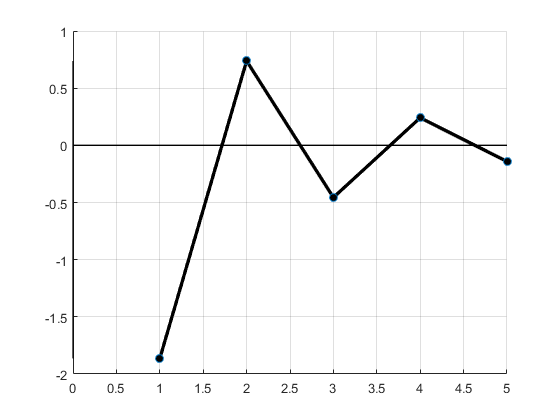
\includegraphics[width=\linewidth]{fp_example/fEvals.png} 
\end{minipage}\hspace{6pt}\vline \hspace{6pt}\begin{minipage}{.45\linewidth}
Si miramos $|f(x)|$ en nuestras propuestas de raices:
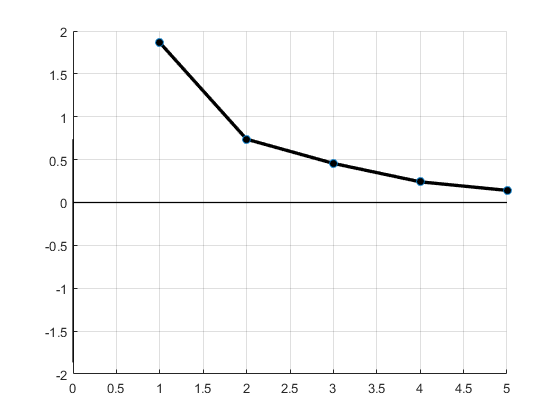
\includegraphics[width=\linewidth]{fp_example/abs_fEvals.png} 
\end{minipage}


\end{frame}


\subsection{Ejemplo 2 Punto Fijo}


\begin{frame}
\frametitle{Otro ejemplo: Punto Fijo}

Supongamos que queremos hallar la raiz de $f(x) = x^2-x-1$



\begin{minipage}{.45\linewidth}
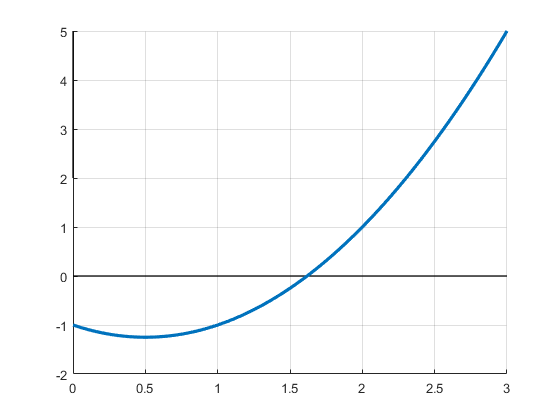
\includegraphics[width=\linewidth]{fp_example2/f.png} 

\end{minipage} $\rightarrow$  \begin{minipage}{.45\linewidth}
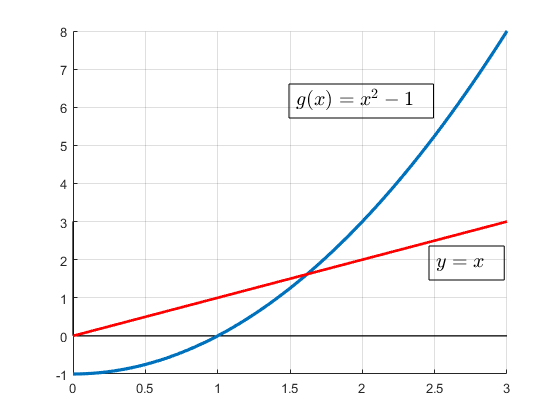
\includegraphics[width=\linewidth]{fp_example2/g.png} 
\end{minipage}

$$g(x) = x^2-1$$
\end{frame}



%iter 1
\begin{frame}
\frametitle{Ejemplo: Punto Fijo}

Supongamos que queremos hallar la raiz de $f(x) = x^2-x-1$,
damos una condición inicial $x_0=2$


\begin{minipage}{.75\linewidth}
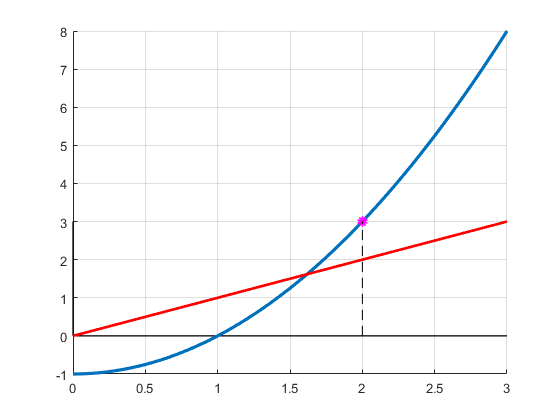
\includegraphics[width=\linewidth]{fp_example2/iter1.png} 

\end{minipage} \begin{minipage}{.2\linewidth}
$$ x_1 = (-2)^2-1 $$
$$ x_1 = 3 $$

\end{minipage}
\end{frame}

%iter 2
\begin{frame}
\frametitle{Ejemplo: Punto Fijo}

Supongamos que queremos hallar la raiz de $f(x) =x^2-x-1$,
damos una condición inicial $x_0=2$


\begin{minipage}{.75\linewidth}
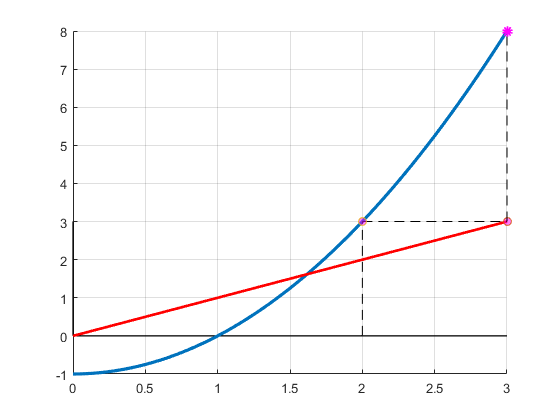
\includegraphics[width=\linewidth]{fp_example2/iter2.png} 

\end{minipage}  \begin{minipage}{.2\linewidth}
$$ x_2 = g(3) = 8$$

\end{minipage}
\end{frame}


%iter 3
\begin{frame}
\frametitle{Ejemplo: Punto Fijo}

Supongamos que queremos hallar la raiz de $f(x) = x^2-x-1$,
damos una condición inicial $x_0=2$


\begin{minipage}{.75\linewidth}
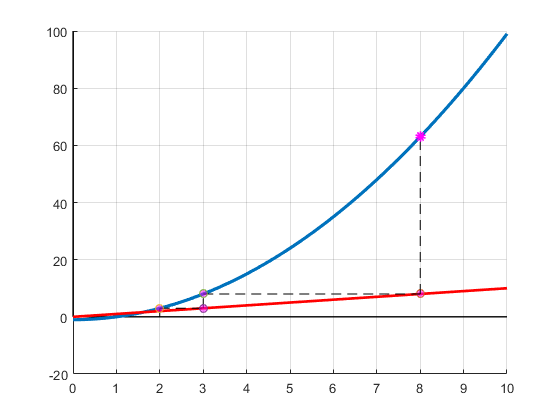
\includegraphics[width=\linewidth]{fp_example2/iter3.png} 

\end{minipage}  \begin{minipage}{.2\linewidth}
$$ x_3 = g(8) = 63$$

\end{minipage}
\end{frame}

\subsection{Convergencia de Punto Fijo}


\begin{frame}
\frametitle{Convergencia de Punto Fijo}

Es posible demostrar (no lo vamos a hacer) que el error real en cada iteración se comporta como:
$$ E_{i+1} = g'(\xi) E_{i}  $$
Para algún $\xi \in [x_{root}, x_i]$ 


De esto puede concluirse que el problema convergerá a la raíz siempre que:
$$\boxed{ |g'(\xi)|<1 } $$
\end{frame}


\section{Newthon-Raphson}

\begin{frame}
\frametitle{Newton-Raphson}
Es uno de los métodos más usados.

\begin{minipage}{.7\linewidth}
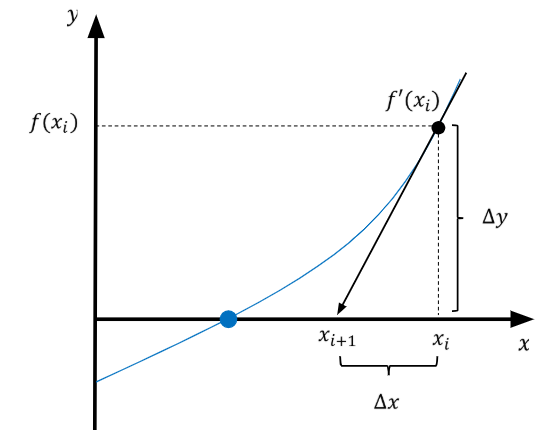
\includegraphics[width=\linewidth]{NewthonRaphson/NR.PNG} 
\end{minipage} \pause \begin{minipage}{.2\linewidth}

$$f'(x_i) = \frac{f(x_i)}{x_{i+1}-x_i}  $$

\begin{equation}
\label{eq:nr}
x_{i+1} = x_i - \frac{f(x_i)}{f'(x_i)} 
\end{equation}
\end{minipage}

\end{frame}

\subsection{NR un ejemplo}


\begin{frame}
	\frametitle{Newton-Raphson: un ejemplo}

Supongamos que queremos hallar la raiz de $f(x) = e^{-x} -x$


\begin{minipage}{.7\linewidth}
\includegraphics[width=\linewidth]{nr_example/f.png} 

\end{minipage}  \begin{minipage}{.25\linewidth}

\textbf{La derivada:}
$$ f'(x) = -e^{-x} - 1$$
	\end{minipage}
\end{frame}

%iter 1
\begin{frame}
	\frametitle{Newton-Raphson: un ejemplo}

Supongamos que queremos hallar la raiz de $f(x) = e^{-x} -x$,
damos una condición inicial $x_0=2$


\begin{minipage}{.7\linewidth}
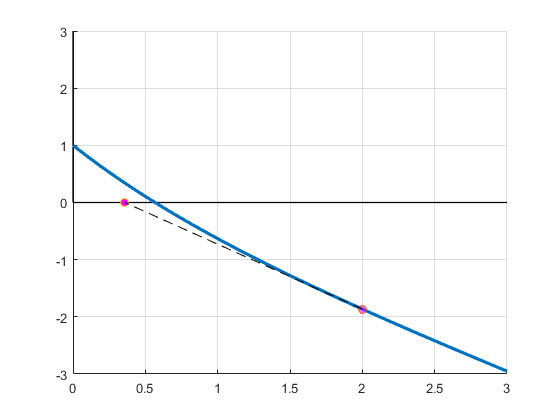
\includegraphics[width=\linewidth]{nr_example/iter1.png} 

\end{minipage}  \begin{minipage}{.25\linewidth}

$$ x_1 = x_0 - \frac{f(2)}{f'(2)}$$
$$ x_1 = 0.3576$$
\end{minipage}

\end{frame}


%iter 2
\begin{frame}
	\frametitle{Newton-Raphson: un ejemplo}

Supongamos que queremos hallar la raiz de $f(x) = e^{-x} -x$,
damos una condición inicial $x_0=2$


\begin{minipage}{.7\linewidth}
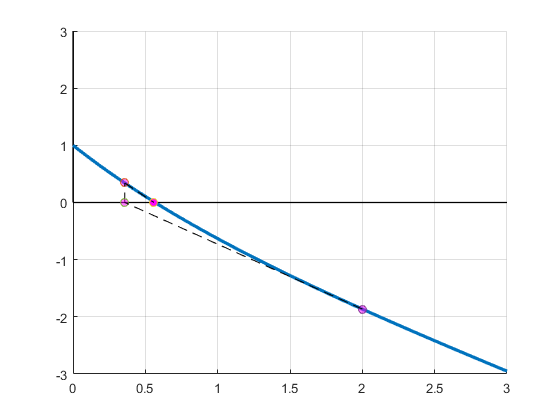
\includegraphics[width=\linewidth]{nr_example/iter2.png} 

\end{minipage}  \begin{minipage}{.25\linewidth}

$$ x_1 = 0.3576$$
$$ x_2 = x_1 - \frac{f(x_1)}{f'(x_1)}$$
$$ x_1 = 0.5587$$
\end{minipage}
\end{frame}


\begin{frame}
	\frametitle{Newton-Raphson: un ejemplo}
Si hacemos un zoom:

\begin{minipage}{.8\linewidth}
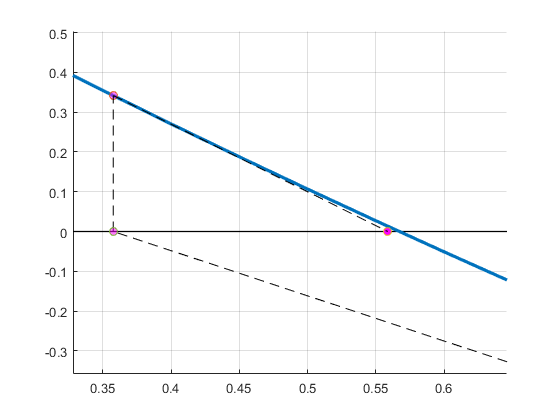
\includegraphics[width=\linewidth]{nr_example/iter2_zoom.png} 
\end{minipage} 
\end{frame}


\subsection{NR ejemplo 2}

\begin{frame}
\frametitle{Otro ejemplo: Newton-Raphson}

Supongamos que queremos hallar la raiz de $f(x) = x^2-x-1$



\begin{minipage}{.7\linewidth}
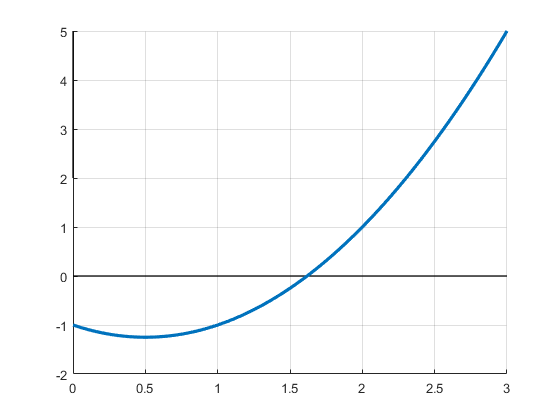
\includegraphics[width=\linewidth]{fp_example2/f.png} 

\end{minipage} \begin{minipage}{.25\linewidth}
\textbf{La derivada:}
$$ f'(x) = 2x -1$$ 
\end{minipage}

\end{frame}


%iter 1
\begin{frame}
	\frametitle{Otro ejemplo: Newton-Raphson}

Supongamos que queremos hallar la raiz de $f(x) = x^2-x-1$,
damos una condición inicial $x_0=2$


\begin{minipage}{.7\linewidth}
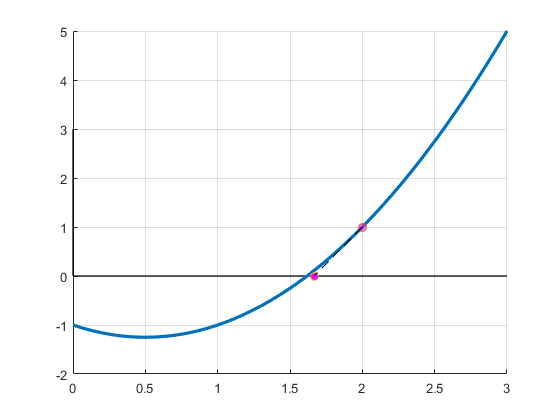
\includegraphics[width=\linewidth]{nr_example2/iter1.png} 

\end{minipage}  \begin{minipage}{.25\linewidth}

$$ x_1 = x_0 - \frac{f(2)}{f'(2)}$$
$$ x_1 = 1.6667$$
\end{minipage}

\end{frame}


%iter 2
\begin{frame}
	\frametitle{Otro ejemplo: Newton-Raphson}

Supongamos que queremos hallar la raiz de $f(x) = x^2-x-1$,
damos una condición inicial $x_0=2$


\begin{minipage}{.7\linewidth}
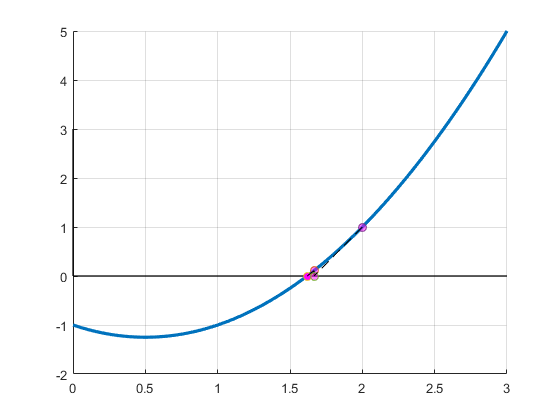
\includegraphics[width=\linewidth]{nr_example2/iter2.png} 

\end{minipage}  \begin{minipage}{.25\linewidth}
$$ x_1 = 1.6667$$
$$ x_2 = x_1 - \frac{f(x_1)}{f'(x_1)}$$
$$ x_2 = 1.6190$$
\end{minipage}

\end{frame}

\begin{frame}
	\frametitle{Otro ejemplo: Newton-Raphson}
Si hacemos un zoom:

\begin{minipage}{.8\linewidth}
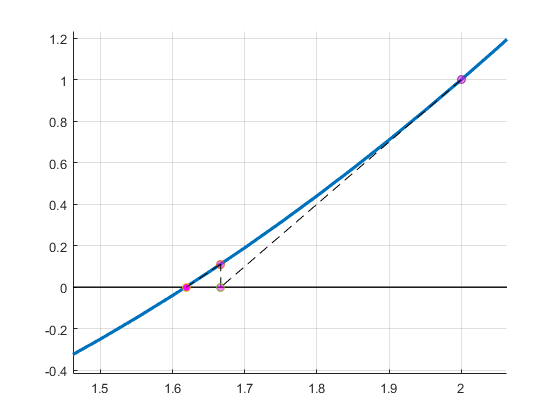
\includegraphics[width=\linewidth]{nr_example2/iter2_zoom.png} 
\end{minipage} 
\end{frame}

\subsection{Consideraciones}
\begin{frame}
\frametitle{Newton-Raphson: Consideraciones}
\begin{minipage}{.45\linewidth}
\begin{itemize}
\item Es un método poderoso.
\item No siempre converge.
\item Requiere poder computar la derivada de la función (costoso).
\end{itemize}

\end{minipage} \begin{minipage}{.45\linewidth}
\textbf{Ejemplo de no convergencia}

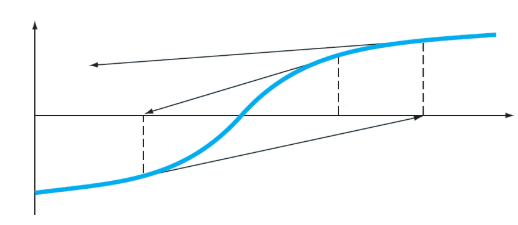
\includegraphics[width=\linewidth]{NewthonRaphson/divergencia.PNG} 
\end{minipage}
\end{frame}


\section{Método de la secante}

\begin{frame}
\frametitle{Método de la Secante}
Deriva de Newton-Raphson, aproximando la derivada:

\begin{minipage}{.55\linewidth}
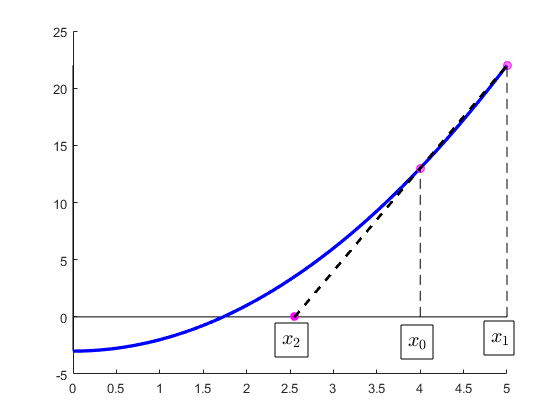
\includegraphics[width=\linewidth]{sec_example/draw.PNG} 
\end{minipage} \begin{minipage}{.4\linewidth}
$$f'(x_{i}) \approx \frac{f(x_{i-1})-f(x_i)}{x_{i-1}-x_i}$$ 
Si utilizamos esto en la ecuación \ref{eq:nr} obtendremos:

$$\boxed{x_{i+1} =x_i - \frac{f(x_i)(x_{i-1}-x_i)}{f(x_{i-1})-f(x_i)} }$$
\end{minipage}
\end{frame}

\subsection{Secante un ejemplo}

\begin{frame}
\frametitle{Método de la secante: un ejemplo}

Supongamos que queremos hallar la raiz de $f(x) = x^2-x-1$



\begin{minipage}{.7\linewidth}
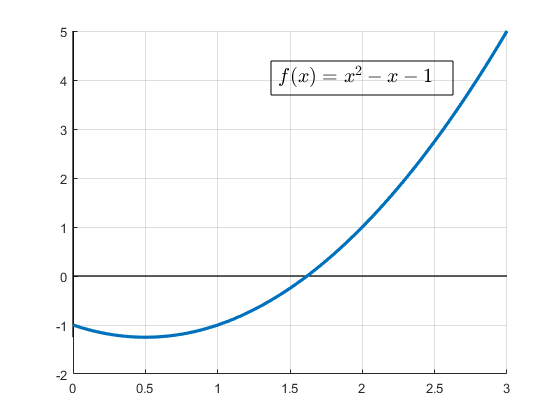
\includegraphics[width=\linewidth]{sec_example/f.png} 

\end{minipage} \begin{minipage}{.25\linewidth}
\end{minipage}

\end{frame}


%iter 1
\begin{frame}
\frametitle{Método de la secante: un ejemplo}

Supongamos que queremos hallar la raiz de $f(x) = x^2-x-1$,
damos una condición inicial $x_{-1}=2.1,x_0=2$


\begin{minipage}{.7\linewidth}
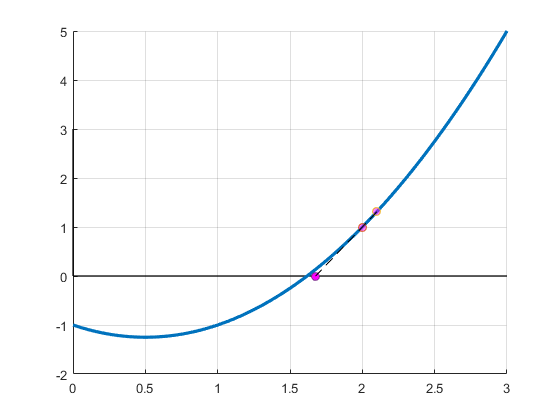
\includegraphics[width=\linewidth]{sec_example/iter1.png} 

\end{minipage}  \begin{minipage}{.25\linewidth}

$$ x_1 = 2 - \frac{f(2)(2.1-2)}{f(2.1)-f(2)}$$
$$ x_1 = 1.6774$$
\end{minipage}

\end{frame}


%iter 2
\begin{frame}
	\frametitle{Método de la secante: un ejemplo}

Supongamos que queremos hallar la raiz de $f(x) = x^2-x-1$,
damos una condición inicial $x_{-1}=2.1,x_0=2$


\begin{minipage}{.7\linewidth}
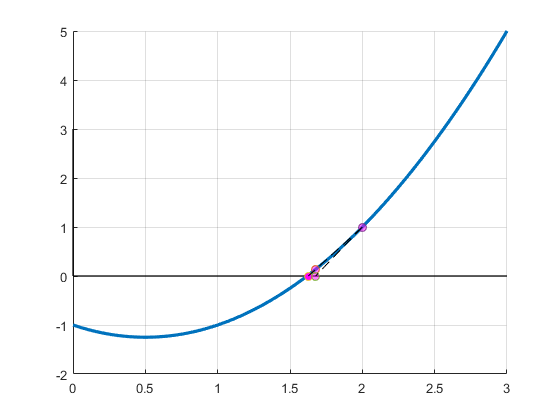
\includegraphics[width=\linewidth]{sec_example/iter2.png} 

\end{minipage}  \begin{minipage}{.25\linewidth}
$$ x_1 = 1.6667$$
$$ x_2 = x_1 -\frac{f(x_1)(x_0-x_1)}{f(x_0)-f(x_0)}$$
$$ x_2 = 1.6265$$
\end{minipage}

\end{frame}

\begin{frame}
	\frametitle{Método de la secante: un ejemplo}
Si hacemos un zoom:

\begin{minipage}{.8\linewidth}
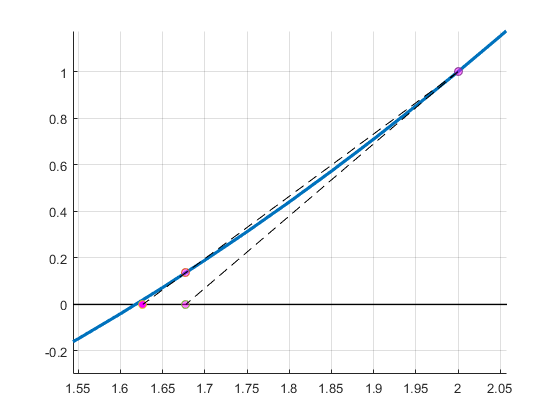
\includegraphics[width=\linewidth]{sec_example/iter2_zoom.png} 
\end{minipage} 
\end{frame}

\subsection{Método de la secante: Consideraciones}

\begin{frame}
\frametitle{Método de la secante: Consideraciones}

\begin{itemize}
\item El método no utiliza el cálculo de la derivada.
\item Requiere de 2 condiciones iniciales.
\item Estas 2 condiciones iniciales pueden estar en el mismo lado de la raiz (a diferencia de \textit{bracketing methods}).
\end{itemize}

\end{frame}




\end{document}

%%% Local Variables: 
%%% mode: latex
%%% TeX-master: t
%%% End: 







